\section{Introduction}

%%%%%%%%%%%%%%%%%%%%%%%%%%%%%%%%%%%%%%%%%%%%%%%%%%%%%%%%%%%%%%%%%%%%%%%%%%%%%%%%%%%%
\subsection{Problem Background}%第一部分 问题背景

\indent\indent  With the emergence of ride-hailing companies like Didi Chuxing and Uber, people are increasingly inclined to travel by taxi. Providing users with suitable driving routes based on their preferences is an important aspect of enhancing the user experience. Historical data indicates that the shortest distance or travel time may not necessarily be the most appropriate route. The user's preferences seem to be influenced by various other factors.\\
\indent Due to the ambiguity of evaluation metrics, it is challenging to find a universally applicable evaluation method for automatically selecting the optimal path. Therefore, we need to extract user preference information from historical data and give the selection weights for different routes. It will be used for future route selection, which is of importance for the development of taxi companies.

%%%%%%%%%%%%%%%%%%%%%%%%%%%%%%%%%%%%%%%%%%%%%%%%%%%%%%%%%%%%%%%%%%%%%%%%%%%%%%%%%%%%
\subsection{Restatement of the Problem}%第二部分 问题重述

\indent\indent Having understood the problem, we figure out the following tasks:
\begin{itemize}
    \item \textit{Task 1}: According to the computational method of SIM, we aim to determine \textbf{the maximum value of SIM in Example 1} and \textbf{find a set of weights for each edge in the directed weighted graph}.
    \item \textit{Task 2}: Based on the data file given in the question,we \textbf{treat the length of the edges as the weights of the roads} without considering historical data and user preferences. And we need to \textbf{calculate the SIM value in Case 1}.
    \item \textit{Task 3}: We need to design a model that can \textbf{determine the weights of each edge in any given graph} in order to maximize the SIM value. Once the model is designed, we will apply it to Case 1 mentioned and showcase the maximum SIM value.
    \item \textit{Task 4}: The weight values provided by our designed model should differ from the edge lengths. We need to explain \textbf{the difference between the two} and demonstrate through how the weight values we provide, compared to the edge lengths, offer advantages in terms of path selection.
\end{itemize}

%%%%%%%%%%%%%%%%%%%%%%%%%%%%%%%%%%%%%%%%%%%%%%%%%%%%%%%%%%%%%%%%%%%%%%%%%%%%%%%%%%%%
\subsection{Previous Reserach}%第三部分 过往的研究

\indent\indent This problem essentially belongs to ISPL problem in inverse combinatorial optimization. It requires us to optimize and determine accurate edge weights from partially defined information such as historical data. The objective is to ensure that the maximum number of paths coincide with the shortest path, resulting in the maximum SIM value. Prior to this, a considerable number of scholars have conducted research in this area. \\
\indent Burton and Toint were among the pioneering researchers in the study of the inverse shortest path problem. They specialized the binary quadratic programming method proposed by Goldfarb and Idnani in 1983. And subsequently, the problem was regarded as a linear programming model. Research revealed that the problem could be transformed into a minimum-cost cycle problem and could not be solved using polynomial algorithms. Cai and Yang addressed the ISPP problem in 1994, and since then, several algorithms have been proposed, including those based on linear and bilinear programming models (Ahmed and Guan, 2004) and genetic algorithms (António Leitão, Adriano Vinhas, Penousal Machado, Francisco Câmara Pereira, 2017) to solve the ISPL problem. Therefore, based on the reference to previous methods, we ultimately chose to use the simulated annealing algorithm to solve this problem. 

%%%%%%%%%%%%%%%%%%%%%%%%%%%%%%%%%%%%%%%%%%%%%%%%%%%%%%%%%%%%%%%%%%%%%%%%%%%%%%%%%%%%
\subsection{Our Work}%第四部分 介绍我们团队的工作

\indent\indent For convenience, we draw a flow chart to better represent our work:
\begin{figure}[H]
    \centering
    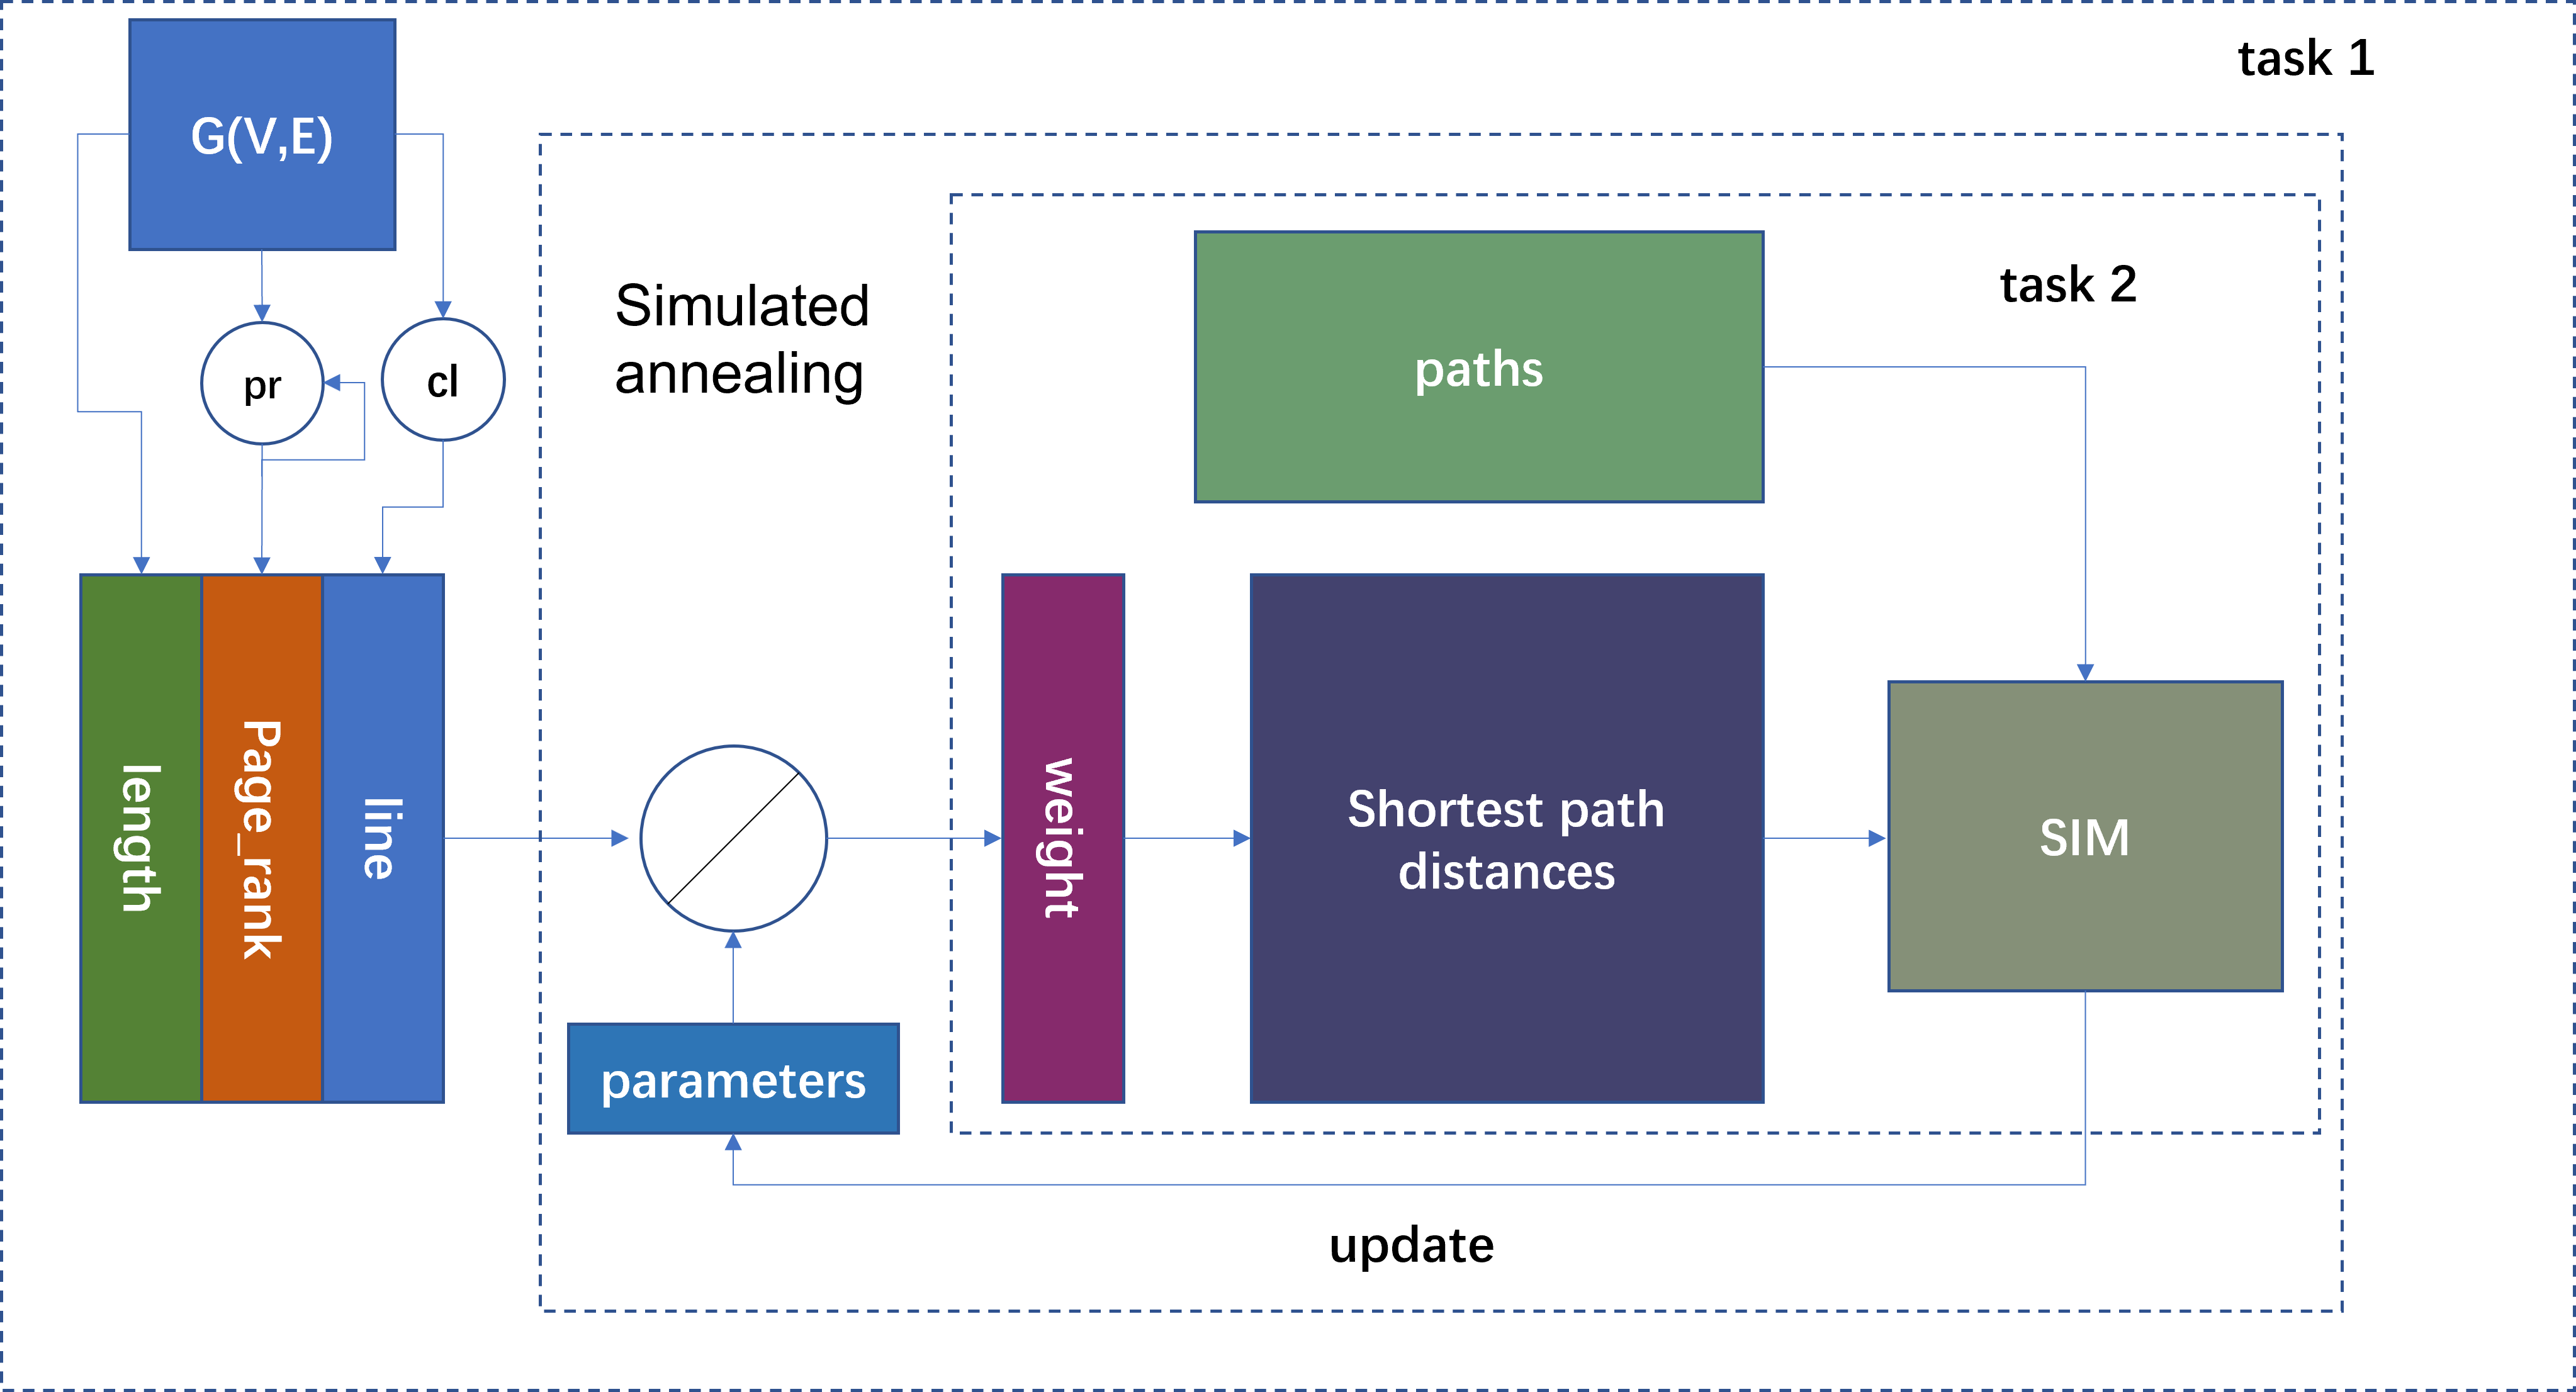
\includegraphics[width=12cm,height=9cm]{核心思路.png}
    \caption{Our Mind Map for tasks}
\end{figure}
\begin{itemize}
    \item Based on the given information that the SIM value in Example 1 is used to determine whether four paths belong to the shortest paths, it can only take five values: 0, 0.25, 0.5, 0.75, and 1. We begin by proving that in Example 1, the SIM value cannot be equal to 1. Secondly, we find a set of edge weights that result in a SIM value of 0.75 and verify it using a computer program. Therefore, we conclude that \textbf{the maximum value for the SIM value is 0.75}.
    \item We utilized the Dijkstra's algorithm to establish a model for calculating the SIM value of a known weighted graph. We constructed a weighted directed graph using the provided data of points and edges in Case 1. Then, for the given choices of the starting and ending points for path selection, we computed the shortest path and analyzed whether the length of each given path was equal to the minimum length. We also calculated the percentage of paths that satisfied this condition.Based on the analysis we conducted for Case 1, we obtained a \textbf{SIM value of 0.248971}.
    \item We first proposed factors to measure the road weight: \textbf{road length, road importance, and the straight-line distance}. Drawing inspiration from PageRank, we introduced \textbf{the edge PageRank value} to determine the importance of roads. We calculated the straight-line distance of roads based on the weighted sum of the squared latitude and longitude differences between the road's starting and ending points, considering the impact of taking detours on customer preferences. Based on this, we designed a model with \textbf{simulated annealing algorithm} and substituted the data from Case 1 into the models to determine the parameters. In the model, we explicitly considered the straight-line distance between the starting and ending points, \textbf{with the  maximum SIM value of 0.273278}. Then, we optimized the calculation of edge PageRank by incorporating the straight-line distance and the objective positions of the starting and ending points. We then obtained \textbf{the maximum SIM values of 0.298223 for Case 1}.
    \item We calculated the weights of each edge and used two different models to \textbf{increase the original SIM value by 9.76298\% and 19.7822\%  respectively}.We plotted the edge weights against the edge lengths in a scatter plot and analyzed the corresponding relationship between them, proposing possible reasons for it. We also analyzed the relationship between \textbf{the indicator of road importance (PageRank) and edge length}, and examined how it influences the final edge weights.
\end{itemize}


